To be able to understand the method, we will introduce a few theoretical 
backgrounds that are related to the tools I will use in this research.
\section{Molecular Dynamics Simulation}
As mentioned in the previous chapter, molecular dynamics simulation is 
a numerical system that describe atomic status over time in a specified 
environment. From the cultivated information, we can either investigate 
the atomic behaviors or calculate thermophysics properties such as thermal 
conductivity and viscosity easily. A standard molecular dynamics simulation 
has an algorithm as follows \cite{manjunatha_development_2018}
\begin{figure}
    \begin{center}
        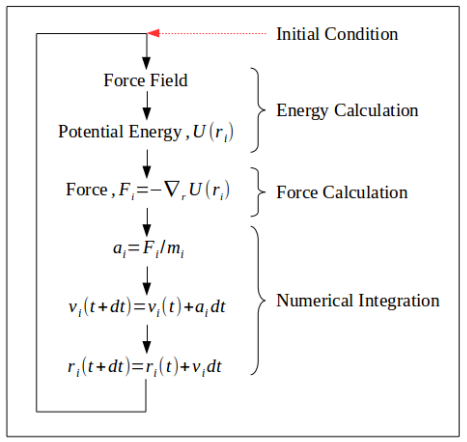
\includegraphics[width=0.75\textwidth]{mdalgo.png}
    \end{center}
    \caption{Basic outline of a MD simulation}
\end{figure}
\newpage
The initial conditions describe the initial state of the atoms such as 
velocity $v(t_0)$, mass of atom $m$ and coordination $r(t_0)$. For atoms of a liquid, given the $i^{th}$ atom, 
the initial coordination $r_i(t_0)$ is randomized along with several 
constraints such as structural constraints (angles, bond lengths) 
and displacement constraints to avoid malfunction in the system as well as 
systematic errors. The initial velocity $v_i(t_0)$ is randomized on the Gaussian 
distribution with the constraint that the total momentum of the entire system 
is $0$.

After the initial setup, a class of functions called a force field is used 
to calculate the potential energy $U_i = U(r_i)$ which is a function of position 
that obeys the structural constraints of the atom. The obtained potential 
energy $U(r_i)$ can be used to deduce the forces $F_i$ that apply on the atom.

The force $F_i$ is then processed by using Verlet algorithm as follows to obtain 
the functions of velocity and position over time. For a time step $\Delta t$, 
the function that presents the position of the $i^{th}$ atom after $\Delta t$ is
\begin{equation}
    r_{i}(t+\Delta t) \approx r_{i}(t)+\Delta t \dot{r}_{i}(t)+\frac{1}{2} \Delta t^{2} \ddot{r}_{i}(t)\label{eq:2.1.1}
\end{equation}
To get the velocity term after a time step $\Delta t$, we have to deduce $r_i(t)$ 
backwards from $r_i(t+\Delta t)$. Thus
\begin{equation}
    r_{i}(t) \approx r_{i}(t+\Delta t)-\Delta t \dot{r}_{i}(t+\Delta t)+\frac{1}{2} \Delta t^{2} \ddot{r}_{i}(t+\Delta t)\label{eq:2.1.2}
\end{equation}
Substituting \ref{eq:2.1.2} into \ref{eq:2.1.1} we get
\begin{equation}
    \dot{r}_{i}(t+\Delta t)=\dot{r}_{i}(t)+\frac{1}{2} \Delta t\left[\ddot{r}_{i}(t)+\ddot{r}_{i}(t+\Delta t)\right]
\end{equation}
Or
\begin{equation}
    \dot{r}_{i}(t+\Delta t)=v_{i}(t+\Delta t)=v_{i}(t)+\frac{1}{2 m_{i}} \Delta t\left[F_{i}(t)+F_{i}(t+\Delta t)\right]
\end{equation}
The values of positions and velocities at $t+\Delta t$ will be served as the next 
initial condition for the next loop of calculation until the set running time 
T is reached. The values of positions and velocities will be used to calculate 
thermal conductivity and viscosity by using a deduction of the Green-Kubo 
relation.
\section{Green-Kubo Relation}
Green-Kubo relation is a formula that shows the relationship between the 
transport coefficient and the dynamical variables. 
The general expression is as follows \cite{hansen_theory_2013}
\begin{equation}
    K=C \int_{0}^{\infty}\langle D(t) D(0)\rangle \mathrm{d} t
\end{equation}
Where K is the transport coefficient, 
D is dynamical variable terms 
and C is the function constant. To be able to calculate viscosity and 
thermal conductivity values, the Green-Kubo expression will be transformed, 
without detailed derivation delivered, and presented as follows
\subsection{Viscosity}
The Green-Kubo expression for calculating viscosity is as follows:
\begin{equation}
    \eta=\frac{V}{k_{b} T} \int_{0}^{\infty}\left\langle P_{\alpha \beta}(t) \cdot P_{\alpha \beta}(0)\right\rangle d t
\end{equation}
Where $P$ is stress tensor terms, 
$\alpha,  \beta \in (x, y, z)$ is the 3D direction, 
V is the system volume, 
T is the system temperature, 
$k_B=1.38 \times 10^{-23}$ $[m^2\cdot kg\cdot s^{-2}\cdot K^{-1}]$ is the Boltzmann constant 
and $\langle \rangle$ is the ensemble average \cite{hansen_theory_2013}.\\
Furthermore, the stress tensor terms can also be expressed as follows:
\begin{equation}
    P_{\alpha \beta}=\frac{1}{V}\left(\sum_{i} m_{i} v_{i_{\alpha}} v_{i_{\beta}}+\sum_{i} r_{i_{\alpha}} f_{i_{\beta}}\right)
\end{equation}
Where $m$ is the atom mass, $v$ is the atom velocity, $r$ is the atom position, 
$f$ is the forces act on atom and $i$ is the atom index \cite{allen_time_2017}.
\subsection{Thermal Conductivity}
The Green-Kubo expression for calculating thermal conductivity is as follows:
\begin{equation}
    \lambda_{T}=\frac{V}{k_{\mathrm{B}} T^{2}} \int_{0}^{\infty} \mathrm{d} t\left\langle J_{\alpha}(t) J_{\alpha}(0)\right\rangle
\end{equation}
Additionally, J is heat flux terms, 
V is the system volume, 
T is the system temperature, 
$k_B=1.38 \times 10^{-23}$ $[m^2\cdot kg\cdot s^{-2}\cdot K^{-1}]$ is the Boltzmann constant, 
$\langle \rangle$ is the ensemble average and
$\alpha \in (x, y, z)$ is the 3D direction \cite{hansen_theory_2013}.\\
Furthermore, The heat flux terms can be broken down further. Thus,
\begin{equation}
    J_{\alpha}=\frac{1}{V}\left(\sum_{i} e_{i} v_{i}+\sum_{i<j}\left(f_{i j} \cdot v_{j}\right) r_{i j_{\alpha}}\right)
\end{equation}
Where $e$ is energy per-atom, 
$v$ is the velocity of atoms, 
$f$ is the force between atoms, 
$r$ is the distance between atoms in the $\alpha$ direction and 
$i$ and $j$ are the atom indices \cite{manjunatha_development_2018}.
\section{eXtreme Gradient Boosting Method}
eXtreme Gradient Boosting (XGBoost) method is a robust supervised machine 
learning method that consists of different advanced statistical techniques. 
The advanced statistical techniques help XGBoost achieve a high calculation 
speed and accuracy. To be able to understand XGBoost for the purpose of this 
research, the following XGBoost component techniques will be explained\\
- Gradient boosting\\
- Regularization object\\
- Sub-sample \& sub-column
\subsection{Gradient Boosting}
The gradient boosting feature improves the accuracy of model prediction 
ability and calculation speed. Gradient boosting consists of 2 parts: 
boosting and gradient.
\subsubsection*{Boosting}
From a mathematical perspective, the boosting algorithm is similar to the 
Lagrange Multiplier method. Given a sample data set of n elements to make 
the XGBoost model, the mission of boosting is to minimize the loss function
$\sum_{i=1}^{n} l\left(y_{i}, \hat{y_{i}}\right)$, 
which is the total sum of differences between predicted values and actual 
values, so that the predicted outcomes are closest to the actual values. 
The boosting algorithm also involves creation of multiple sub-functions from 
given variables which serve as constraints for the Lagrange problem. Finally, 
boosting algorithm takes an adjustable coefficient as the Lagrange Multiplier 
coefficients. Instead of having many coefficients as is typically used in the 
Lagrange multiplier method, boosting only uses a unified coefficient to avoid 
unnecessary complexity for the system while it does not have to compromise too 
much on accuracy. The boosting algorithm can be represented by the following 
expression, where $\hat{f}_b(x)$ represents each sub-function that boosting creates and 
$\lambda$ represents the Lagrange coefficient:
\begin{equation}
    0 \leftarrow \sum_{b=1}^{B} \sum_{i=1}^{n} l\left(r_{i}, \hat{r}_{i}\right)_{b}+\sum_{b=1}^{B} \lambda \hat{f}_{b}(x)
\end{equation}
Which can be written as:
\begin{equation}
    0\leftarrow \sum_{i=1}^{n} l\left(y_{i}, \hat{y}_{i}\right)+\sum_{b=1}^{B} \lambda \hat{f}_{b}(x)
\end{equation}
Furthermore, B is the total number of sub-functions, n is the number of data 
in the sample data and r is the difference between actual values and predicted 
values of the previous sub-function. For example, for any data point i in the 
data sample being processed by sub-function b:
$r_{i}^{b}=y_i^{(b-1)}-\hat{y}_i^{(b-1)}$. 
Initially, $r_{i}^{0}=y_i$ \cite{james_introduction_2013}.
\subsubsection*{Gradient}
Instead of $\sum_{i=1}^{n} l\left(y_{i}, \hat{y_{i}}\right)$, the loss function
is expanded by the Taylor expansion to the second degree, which is where the terms 
“gradient” comes from. Thus, at any $t^{th}$ sub-function, the loss function becomes:
\begin{equation}
    \sum_{i}^{n_{t}}\left[l\left(r_{i}, \hat{r}_{i}^{(t-1)}+\hat{f}_t\left(x_{i}\right)\right)]\right.
\end{equation}
\begin{equation}
    \sum_{i=1}^{n_t}\left[l\left(r_{i}, \hat{r}^{(t-1)}\right)+g_{i} \hat{f}_t\left(\mathbf{x}_{i}\right)+\frac{1}{2} h_{i} {\hat{f}_{t}^{2}}\left(\mathbf{x}_{i}\right)\right]
\end{equation}
Where $g_{i}=\partial_{\hat{r}^{(t-1)}} l\left(r_{i}, \hat{r}^{(t-1)}\right)$ and
$h_i=\partial_{\hat{r}^{(t-1)}}^{2} l\left(r_{i}, \hat{r}^{(t-1)}\right)$ are 
the Taylor expansion coefficients. By expanding into 2nd degree of Taylor expansion, 
the loss function will converge faster and more accurately while avoiding 
overfitting \cite{chen_xgboost:_2016}.\\
Overfitting refers to the performance of a model that is particularly good for a specific set 
of data and consequently may not be able to produce reliable predictions. 
\subsection{Regularization Object}
Regularization is a technique that identifies unnecessary or less important 
variables by shrinking the coefficient of all variables (the coefficients 
inside the sub-functions, which are different from the Lagrange coefficient) 
towards zero. The coefficients of unnecessary or less important variables will 
become zero, thus, do not affect the model \cite{james_introduction_2013}. To control 
the regularization process, the XGBoost method has 2 parameters, the LASSO 
parameter \cite{tibshirani_regression_1996} and the Ridge Regression parameter \cite{hoerl_ridge_1970}.
\subsection{Subsample \& Subcolumn}
Machine learning techniques normally use a set of sample data (training data) 
to create the component functions. However, using the entire training data set 
often encounters overfitting problems. Thus, XGBoost introduces sub-sample and sub-column features.

Sub-sample is a technique that instead of using the entire training data set, 
the algorithm only uses a portion of it.
Sub-column is similar to sub-sample but instead of using a part of training data, 
the algorithm uses a subset of the available variables.
Thus, for each sub-function, a different set of sub-sample and sub-column will 
be implemented. By doing so, the algorithm can prevent overfitting and detect 
the relationship between variables and outcomes even further and use of 
sub-columns also increase the computing speed \cite{chen_xgboost:_2016}.

Corresponding to the explained theory, XGBoost has the following parameters 
that need to be chosen:\\
- n\_estimators = number of sub-functions B\\
- learning\_rate = the Lagrange coefficient $\lambda$\\
- subsample = sub-sample size\\
- colsample\_bytree = sub-column size\\
- reg\_alpha = the LASSO parameter\\
- reg\_lambda = the Ridge Regression parameter


\section{Cross Validation}
Every predictive model for a purpose comes along with a prediction error 
(true error), which show how different the outputs of the model compared 
to the true values of the corresponding inputs. Cross validation is a method 
that estimates the true error of a predictive model. For sample data, which 
includes both input and true values of output, the estimation of error is a 
simple job. However, for real data, the true error is usually unable to be 
found due to the absence of the true values of output. Thus, cross validation 
is implemented to approximate the true error from existing data sets 
\cite{rodriguez_sensitivity_2010}.
\subsection*{k-folds method}
The k-folds method is a cross validation method that’s popularly used in 
machine learning because of its good performance. In the k-fold method, 
the sample data set of n data points is divided into k equal $\frac{n}{k}$ data point 
portions with no shared component. The ith portion will be used to test the 
model (validation set) and give a numerical test error while the other k-1 
portions will be used to train the model (training set). The process iterates 
k times so that every portion would be selected as test set once. The true 
error of the model will be estimated by averaging k numerical values of test 
error. The error measuring error for numerical output problem can be mean 
square error method as follows:
\begin{equation}
    M S E=(y-\hat{y})^{2}
\end{equation}
Where $y$ is the real value and $\hat{y}$ is the predicted value. Thus, the 
true error estimation becomes
\begin{equation}
    True Error Estimation=\frac{1}{k} \sum_{i=1}^{k} \sum_{j=1}^{n_i}\left(y_{j}-\hat{y}_{j}\right)_{i}^{2}
\end{equation}
Where i is the index of divided portions, j is the index of data points and 
$n_i$ is the data in the $i^{th}$ portion. The k-folds method helps us to 
reduce the variance of models’ training scores, which due to the splitting of 
validation set and training set, and estimate the most stable performance scores.